\documentclass[11pt]{article}
%\usepackage{fullpage,graphicx,algorithm,algorithmic,bm,amsmath,amsthm,amssymb,color,hyperref,cite,natbib}

% if you need to pass options to natbib, use, e.g.:
%\PassOptionsToPackage{numbers}{natbib}
\usepackage[numbers]{natbib}
\usepackage{fullpage}
\usepackage{bm,amsmath,amsthm,amssymb,multicol,algorithmic,algorithm,enumitem}
\usepackage{wrapfig,lipsum}
\usepackage[textwidth=1cm,textsize=footnotesize]{todonotes}

% ready for submission
\usepackage{neurips_2020}

\usepackage[colorlinks=true,
linkcolor=red,
urlcolor=blue,
citecolor=blue]{hyperref}
\usepackage{hyperref}
\usepackage{cleveref}
\usepackage{subfigure}
\setlength{\parskip}{.2cm}


\def\M{\mathcal{M}}
\def\A{\mathcal{A}}
\def\Z{\mathcal{Z}}
\def\S{\mathcal{S}}
\def\D{\mathcal{D}}
\def\R{\mathcal{R}}
\def\P{\mathcal{P}}
\def\K{\mathcal{K}}
\def\E{\mathbb{E}}
\def\F{\mathfrak{F}}
\def\l{\boldsymbol{\ell}}

\newtheorem{Fact}{Fact}
\newtheorem{Lemma}{Lemma}
\newtheorem{Prop}{Proposition}
\newtheorem{Theorem}{Theorem} 
\newtheorem{Def}{Definition}
\newtheorem{Corollary}{Corollary}
\newtheorem{Conjecture}{Conjecture}
\newtheorem{Property}{Property}
\newtheorem{Observation}{Observation}
%\theorembodyfont{\rmfamily}
\newtheorem{Exa}{Example}
\newtheorem{assumption}{H\!\!}
\newtheorem{assumptionA}{S\!\!}
\newtheorem{assumptionL}{L\!\!}
\newtheorem{Remark}{Remark}
\newtheorem*{Lemma*}{Lemma}
\newtheorem*{Theorem*}{Theorem}
 \makeatletter
\renewenvironment{proof}[1][\proofname]{%
   \par\pushQED{\qed}\normalfont%
   \topsep6\p@\@plus6\p@\relax
   \trivlist\item[\hskip\labelsep\bfseries#1]%
   \ignorespaces
}{%
   \popQED\endtrivlist\@endpefalse
}
\makeatother

%%%%%%%%%%% Stuffs for Tikz %%%%%%%%%%%%%%%%%%
\usepackage{pgfplots}
\usepackage{xargs}
\usepackage{stmaryrd}
\usetikzlibrary{arrows,shapes,calc,tikzmark,backgrounds,matrix,decorations.markings}
\usepgfplotslibrary{fillbetween}

\pgfplotsset{compat=1.3}

\usepackage{relsize}
\tikzset{fontscale/.style = {font=\relsize{#1}}
    }

\definecolor{lavander}{cmyk}{0,0.48,0,0}
\definecolor{violet}{cmyk}{0.79,0.88,0,0}
\definecolor{burntorange}{cmyk}{0,0.52,1,0}

\def\lav{lavander!90}
\def\oran{orange!30}

\definecolor{asuorange}{rgb}{1,0.699,0.0625}
\definecolor{asured}{rgb}{0.598,0,0.199}
\definecolor{asuborder}{rgb}{0.953,0.484,0}
\definecolor{asugrey}{rgb}{0.309,0.332,0.340}
\definecolor{asublue}{rgb}{0,0.555,0.836}
\definecolor{asugold}{rgb}{1,0.777,0.008}

%%%%%%%%%%%%%%%%%%%%%%%%%%%%%%%%%%%%%


\usepackage{shortcuts_OPT}

%\renewcommand{\textwidth}{5.5in}

% Here's the definition of Sb, stolen from amstex
    \makeatletter
    \def\multilimits@{\bgroup
  \Let@
  \restore@math@cr
  \default@tag
 \baselineskip\fontdimen10 \scriptfont\tw@
 \advance\baselineskip\fontdimen12 \scriptfont\tw@
 \lineskip\thr@@\fontdimen8 \scriptfont\thr@@
 \lineskiplimit\lineskip
 \vbox\bgroup\ialign\bgroup\hfil$\m@th\scriptstyle{##}$\hfil\crcr}
    \def\Sb{_\multilimits@}
    \def\endSb{\crcr\egroup\egroup\egroup}
\makeatother

\newtheoremstyle{k}         %name
    {\baselineskip}{2\topsep}      %space above and below
    {\rm}                   %Body font
    {0pt}{\bfseries}  %Heading indent and font
    {}                      %after heading
    { }                      %head after space
    {\thmname{#1}\thmnumber{#2}.}

\theoremstyle{k}
\newtheorem{q}{Q}
\parindent=0pt

%\newcommand{\eric}[1]{\todo[color=red!20]{{\bf EM:} #1}}
%\newcommand{\erici}[1]{\todo[color=red!20,inline]{{\bf EM:} #1}}
%\newcommand{\belhal}[1]{\todo[color=green!20]{{\bf BK:} #1}}
%\newcommand{\belhali}[1]{\todo[color=green!20,inline]{{\bf BK:} #1}}
%\newcommand{\toco}[1]{\todo[color=yellow!20]{{\bf To:} #1}}



\makeatletter
\DeclareRobustCommand*\cal{\@fontswitch\relax\mathcal}
\makeatother

\begin{document}
\title{OPT-AMSGrad: An Optimistic Acceleration of AMSGrad for Nonconvex Optimization}
%\author{}
\date{\today}

\maketitle


\begin{abstract}
We consider a new variant of AMSGrad. 
AMSGrad \citep{RKK18} is a popular adaptive gradient based optimization algorithm that is widely used in training deep neural networks. 
The new variant assumes that mini-batch gradients in consecutive iterations have some underlying structure, which makes the gradients sequentially predictable. 
By exploiting the predictability and ideas from Optimistic Online Learning, the proposed algorithm can accelerate the convergence and increase sample efficiency.
In the nonconvex case, we establish a $\mathcal{O}\left(\sqrt{d/T} +d/T \right)$ non-asymptotic bound independent of the initialization of the method and in the convex case, we show that our method enjoys a tighter non-asymptotic regret bound under some conditions.
We illustrate the practical speedup on several deep learning models through numerical experiments.
\end{abstract}

\section{Introduction}

Deep learning models have been successful in several applications, from robotics (e.g. \citep{LFDA17}), computer vision (e.g \citep{Rnet16,goodfellow2014generative}), reinforcement learning (e.g. \citep{Atari13}), to natural language processing (e.g. \citep{GMH13}).
With the sheer size of modern data sets and the dimension of neural networks, speeding up training is of utmost importance.
To do so, several algorithms have been proposed in recent years, such as  \textsf{AMSGrad} \citep{RKK18}, \textsf{ADAM} \citep{KB15}, \textsf{RMSPROP} \citep{TH12}, \textsf{ADADELTA} \citep{Z12}, and \textsf{NADAM} \citep{D16}.

All the prevalent algorithms for training deep networks mentioned above combine two ideas: the idea of adaptivity from \textsf{AdaGrad} \citep{DHS11,MS10} and the idea of momentum from \textsf{Nesterov's  Method} \citep{N04} or \textsf{Heavy ball} method \citep{P64}.
\textsf{AdaGrad} is an online learning algorithm that works well compared to the standard online gradient descent when the gradient is sparse.
Its update has a notable feature: it leverages an anisotropic learning rate depending on the magnitude of gradient in each dimension which helps in exploiting the geometry of data. 
On the other hand, \textsf{Nesterov's Method} or \textsf{Heavy ball} Method \citep{P64} is an accelerated optimization algorithm whose update not only depends on the current iterate and current gradient but also depends on the past gradients (i.e. momentum). 
State-of-the-art algorithms like \textsf{AMSGrad} \citep{RKK18} and \textsf{ADAM} \citep{KB15} leverage these ideas to accelerate the training process of highly nonconvex objective functions such as deep neural networks losses.

In this paper, we propose an algorithm that goes further than the hybrid of the adaptivity and momentum approach. 
Our algorithm is inspired by \textsf{Optimistic Online learning} \citep{CJ12,RS13,SALS15,ALLW18}, which assumes that a good \emph{guess} of the loss function in each round of online learning is available, and plays an action by exploiting the guess. 
By exploiting the guess, algorithms in \textsf{Optimistic Online learning} enjoy smaller regret than the ones without exploiting the guess.
We combine the \textsf{Optimistic Online learning} idea with the adaptivity and the momentum ideas to design a new algorithm --- \textsf{OPT-AMSGrad}. 
To the best of our knowledge, this is the first work exploring towards this direction. 
The proposed algorithm not only adapts to the informative dimensions, exhibits momentum, but also exploits a good guess of the next gradient to facilitate acceleration. 
Besides the global analysis of \textsf{OPT-AMSGrad}, we also conduct experiments and show that the proposed algorithm not only accelerates convergence of loss function, but also leads to better generalization performance in some cases.

\section{Preliminaries}\label{sec:prelim}
We begin by providing some background on both online learning and adaptive methods.

\textbf{Notations:} We follow the notations in related adaptive optimization papers \citep{KB15,RKK18}. For any vector $u$, $v \in \mathbb R^{d}$,  $u/v$ represents element-wise division,
$u^{2}$ represents element-wise square, $\sqrt{u}$ represents element-wise square-root.
We denote $g_{1:T}[i]$ as the sum of the $i_{th}$ element of $T$ vectors $g_{1}, g_{2},
\dots, g_{T} \in \mathbb R^{d}$.

\subsection{Optimistic Online learning}
The standard setup of \textsf{Online learning} is that, in each round $t$, an online learner selects an action $w_{t} \in \Theta \subseteq \mathbb R^{d}$, then the learner observes $\ell_{t}(\cdot)$ and suffers loss $\ell_{t}(w_t)$ after the action is committed.
The goal of the learner is to minimize the regret, 
$$\text{Regret}_{T}( \{ w_t \} ):= \sum_{t=1}^T \ell_{t}(w_t) - \sum_{t=1}^T \ell_{t}(w^*)\eqsp,$$
which is the cumulative loss of the learner minus the cumulative loss of some benchmark $w^{*} \in \Theta$.
The idea of \textsf{Optimistic Online learning} (e.g. \citep{CJ12,RS13,SALS15,ALLW18}) is as follows.
In each round $t$, the learner exploits a good guess $m_t(\cdot)$ of the gradient $\nabla \ell_t(\cdot)$ of the loss function to choose an action $w_t$. 
\footnote{Imagine that if the learner would had been known $\nabla \ell_t(\cdot)$ (\ie exact guess) before committing its action, then it would exploit the knowledge to determine its action and consequently minimizes the regret.} 
Consider the \textsf{Follow-the-Regularized-Leader} (\textsf{FTRL}, \citep{H14}) online learning algorithm which update reads
\begin{equation} \label{optFTRL}
\textstyle w_t  = \arg \min_{w \in \Theta} \langle w , L_{t-1} \rangle + \frac{1}{\eta} R(w) \eqsp,
\end{equation}
where $\eta$ is a parameter, $R(\cdot)$ is a $1$-strongly convex function with respect to a norm ($\| \cdot \|$) on the constraint set $\Theta$, and $L_{t-1}:= \sum_{s=1}^{t-1} g_s$ is the cumulative sum of gradient vectors of the loss functions up to $t-1$. It has been shown that FTRL has regret at most $O(\sqrt{\sum_{t=1}^T \| g_t \|_*})$.
The update of its optimistic variant, noted \textsf{Optimistic-FTRL} and developed in \citep{SALS15} reads
\begin{equation} \label{optFTRL}
\textstyle w_t  = \arg \min_{w \in \Theta} \langle w , L_{t-1} + m_t \rangle + \frac{1}{\eta} R(w)\eqsp,
\end{equation}
where $m_{t}$ is the learner's guess of the gradient vector $g_{t}:=\nabla \ell_t(w_t)$.
Under the assumption that loss functions are convex, the regret of \textsf{Optimistic-FTRL} is at most $O(\sqrt{\sum_{t=1}^T \| g_t - m_t \|_*  } )$, which can be much smaller than the regret of \textsf{FTRL} if $m_{t}$ is close to $g_{t}$.
Consequently, \textsf{Optimistic-FTRL} can achieve better performance than $\textsf{FTRL}$.
On the other hand, if $m_t$ is far from $g_t$, then the regret of \textsf{Optimistic-FTRL} is only a constant factor worse than that of its counterpart \textsf{FTRL}. 

We emphasize in Section~\ref{sec:opt} the importance of leveraging a good guess $m_t$ for updating $w_t$ in order to get a fast convergence rate (or equivalently, small regret). We will have a similar argument when we compare \textsf{OPT-AMSGrad} and \textsf{AMSGrad}.

\subsection{Adaptive optimization methods}
%\begin{algorithm}[t]
%\begin{algorithmic}[1]
%\small
%\caption{\textsf{AMSGrad} \citep{RKK18}} \label{alg:amsgrad}
%\STATE Required: parameter $\beta_1$, $\beta_2$, and $\eta_t$. 
%\STATE Init: $w_{1} \in \Theta \subseteq \mathbb R^d $ and $v_{0} = \epsilon 1 \in \mathbb R^{d}$.
%\FOR{$t=1$ to $T$}
%\STATE Get mini-batch stochastic gradient vector $g_t$ at $w_t$.
%\STATE $\theta_t = \beta_1 \theta_{t-1} + (1 - \beta_1) g_t$.
%\STATE $v_t = \beta_2 v_{t-1} + (1 - \beta_2) g_t^2$. 
%\STATE $\hat{v}_t = \max( \hat{v}_{t-1} , v_t )$. 
%\STATE $w_{t+1} = w_t - \eta_t \frac{\theta_t}{ \sqrt{\hat{v}}_t }$.
%\text{ (element-wise division)}
%\ENDFOR
%\end{algorithmic}
%\end{algorithm}

Recently, adaptive optimization has been popular in various deep learning applications due to their superior empirical performance. \textsf{Adam} \citep{KB15} is a very popular adaptive algorithm for training deep nets.
It combines the momentum idea \citep{P64} with the idea of \textsf{AdaGrad} \citep{DHS11},
which has different learning rates for different dimensions, adaptive to the learning process. More specifically, the learning rate of \textsf{AdaGrad} in iteration $t$ for a dimension $j$ is proportional to the inverse of $\sqrt{ \Sigma_{s=1}^t g_s[j]^2 }$, where $g_s[j]$ is the $j$-th element of the gradient vector $g_s$ at time $s$.
\begin{wrapfigure}[11]{r}{.5\linewidth}\vspace{-0.3cm}
\begin{minipage}{\linewidth}
 \algsetup{indent=1em}
\begin{algorithm}[H]
\caption{\textsf{AMSGrad} \citep{RKK18}} \label{alg:amsgrad}
\begin{algorithmic}[1]
\small
\STATE Required: parameter $\beta_1$, $\beta_2$, and $\eta_t$. 
\STATE Init: $w_{1} \in \Theta \subseteq \mathbb R^d $ and $v_{0} = \epsilon 1 \in \mathbb R^{d}$.
\FOR{$t=1$ to $T$}
\STATE Get mini-batch stochastic gradient $g_t$ at $w_t$.
\STATE $\theta_t = \beta_1 \theta_{t-1} + (1 - \beta_1) g_t$.
\STATE $v_t = \beta_2 v_{t-1} + (1 - \beta_2) g_t^2$. 
\STATE $\hat{v}_t = \max( \hat{v}_{t-1} , v_t )$. 
\STATE $w_{t+1} = w_t - \eta_t \frac{\theta_t}{ \sqrt{\hat{v}}_t }$.
\text{ (element-wise division)}
\ENDFOR
\end{algorithmic}
\end{algorithm}\vspace{.1cm}
\end{minipage}\end{wrapfigure}
This adaptive learning rate helps accelerating the convergence when the gradient vector is sparse \citep{DHS11} but, when applying \textsf{AdaGrad} to train deep networks, it is observed that the learning rate might decay too fast \citep{KB15}.
Therefore, \citep{KB15} proposes \textsf{Adam} that uses a moving average of gradients divided by the square root of the second moment of the moving average (element-wise fashion), for updating the model parameter $w$.
A variant, called \textsf{AMSGrad} and detailed in Algorithm~\ref{alg:amsgrad}, has been developed in \citep{RKK18} to fix \textsf{Adam} failures at some online convex optimization problems.
The difference between \textsf{Adam} and \textsf{AMSGrad} lies in line 7 of Algorithm~\ref{alg:amsgrad}.
\textsf{Adam} does not have the max operation on line 7 (i.e. $\hat{v}_t = v_t$ for \textsf{Adam}) while \citep{RKK18} adds the operation to guarantee a non-increasing learning rate,$\frac{\eta_t }{ \sqrt{\hat{v}}_t }$, which helps for the convergence (i.e. average regret $\frac{\text{Regret}_T}{T} \rightarrow 0$).
For the hyper-parameters of \textsf{AMSGrad}, it is suggested in~\citep{RKK18} that $\beta_1=0.9$ and $\beta_2=0.99$.


\section{\textsf{OPT-AMSGrad} Algorithm}\label{sec:opt}
We formulate in this section the proposed optimistic acceleration of AMSGrad, noted \textsf{OPT-AMSGrad}, and detailed in Algorithm~\ref{alg:optamsgrad}.
\begin{algorithm}[H]
\begin{algorithmic}[1] 
\small
\caption{\textsf{OPT-AMSGrad}} \label{alg:optamsgrad}
\STATE Required: parameter $\beta_1$, $\beta_2$, $\epsilon$, and $\eta_t$. 
\STATE Init: $w_1 = w_{-1/2} \in \Theta \subseteq \mathbb R^d $ and $v_{0} = \epsilon 1 \in \mathbb R^{d}$.
\FOR{$t=1$ to $T$}
\STATE Get mini-batch stochastic gradient $g_t$ at $w_t$.
\STATE $\theta_t = \beta_{1} \theta_{t-1} + (1 - \beta_{1}) g_t$.
\STATE $v_t = \beta_2 v_{t-1} + (1 - \beta_2) g_t^{2}$.
\STATE $\hat{v}_t = \max( \hat{v}_{t-1} , v_t )$. 
\STATE $w_{t+\frac{1}{2}} =  w_{t} - \eta_t \frac{\theta_t}{ \sqrt{\hat{v}_t }  } $.
\STATE $w_{t+1} = w_{t+\frac{1}{2}} - \eta_{t} \frac{h_{t+1}}{ \sqrt{\hat{v}_t } } $,  \\  
where $h_{t+1}:= \beta_{1} \theta_{t-1} + (1 - \beta_{1}) m_{t+1}$  and $m_{t+1}$ is the guess of $g_{t+1}$. 
\ENDFOR 
\end{algorithmic}
\end{algorithm}
\begin{wrapfigure}[10]{l}{.5\linewidth}\vspace{-1.0cm}
\begin{minipage}{\linewidth}
\begin{figure}[H]
    \hspace{-0.15in}
    \centering
    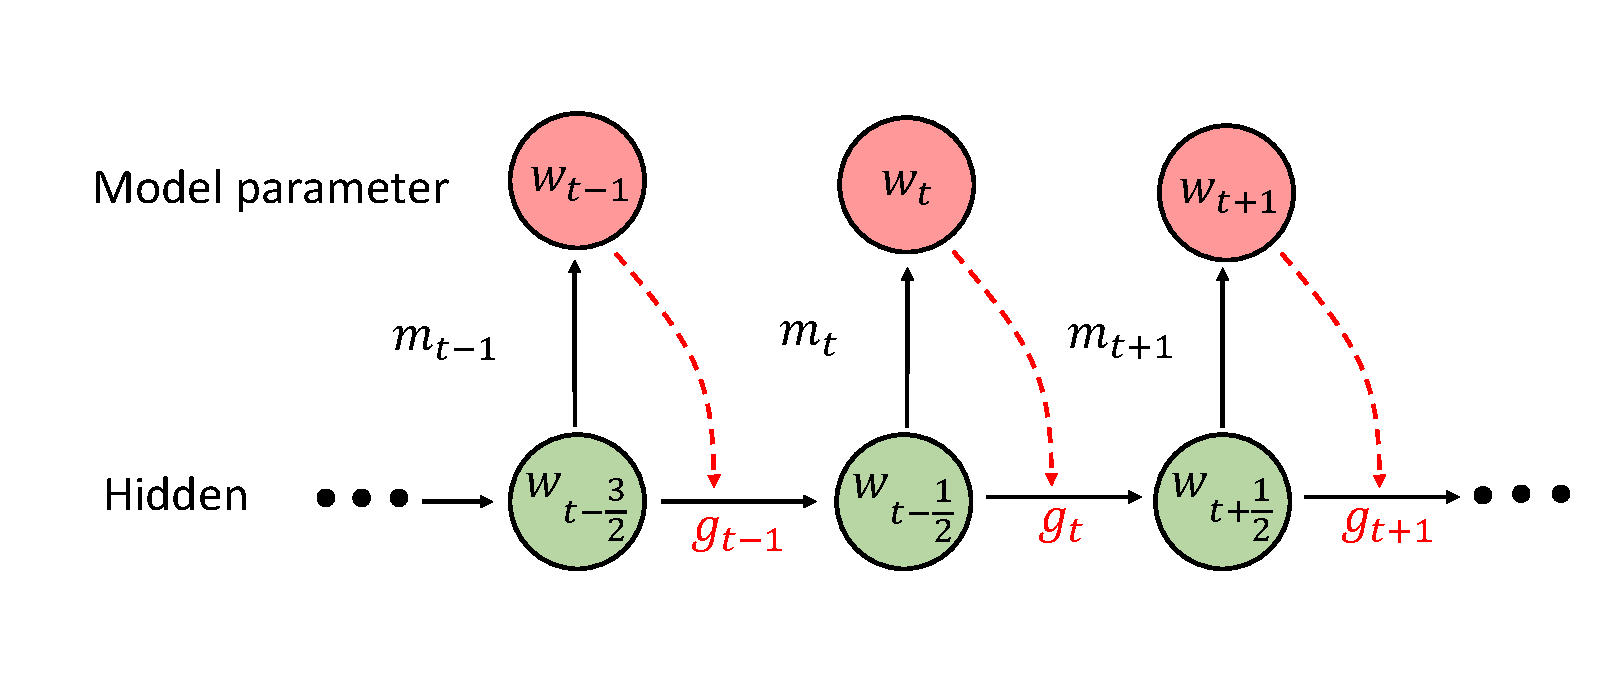
\includegraphics[width=2.7in]{plot.pdf}
    \caption{\textsf{OPT-AMSGRAD}.}
     \label{fig:scheme}
\end{figure}
\end{minipage}\end{wrapfigure}
 It combines the idea of adaptive optimization with optimistic learning. 
At each iteration, the learner computes a gradient vector $g_{t}:= \nabla \ell_t( w_t)$ at $w_{t}$ (line 4), then it maintains an exponential moving average of $\theta_{t} \in \mathbb R^{d}$ (line 5) and $v_{t} \in \mathbb R^{d}$ (line 6), which is followed by the max operation to get $\hat{v}_{t} \in \mathbb R^{d}$ (line 7). 
The learner also updates an auxiliary variable $w_{t+\frac{1}{2}} \in \Theta$ (line 8). 
It uses the auxiliary variable (hidden model) to update and commit $w_{t+1}$ (line 9), which exploits the guess $m_{t+1}$ of $g_{t+1}$ to get $w_{t+1}$.
%As the learner's action set is $\Theta \subseteq \mathbb R^{d}$, we adopt the notation $\Pi_{\Theta}[\cdot]$ for the projection to $\Theta$ if needed. 
We summarize the interplay between the auxiliary structure $w_{t+\frac{1}{2}}$ and the model parameter $w_{t+1}$ of \textsf{AMSGrad} in Figure \ref{fig:scheme}.


The proposed \textsf{OPT-AMSGrad} inherits three properties:
\begin{itemize}
\item Adaptive learning rate of each dimension as \textsf{AdaGrad} \cite{DHS11}. (line 6, line 8 and line 9)
\item Exponential moving average of the past gradients as \textsf{Nesterov's method} \cite{N04} and the \textsf{Heavy-Ball} method \cite{P64}. (line 5)
\item Optimistic update that exploits a good guess of the next gradient vector
as optimistic online learning algorithms \cite{CJ12,RS13,SALS15}. (line 9)
\end{itemize}
The first property helps for acceleration when the gradient has a sparse structure.
The second one is from the well-recognized idea of momentum which can also help for acceleration. 
The last one, perhaps less known outside the \textsf{Online learning} community, can actually lead to acceleration when the prediction of the next gradient is good. This property will be elaborated in the following subsection in which we provide the theoretical analysis of \textsf{OPT-AMSGrad}.
Observe that the proposed algorithm does not reduce to \textsf{AMSGrad} when $m_{t}=0$.
%Furthermore, if $\Theta = \mathbb R^{d}$ (unconstrained case), one might want to combine line 8 and line 9 and get a single line as $w_{t+1}=
%w_{t} - \eta_t \frac{\theta_t + h_{t+1}}{ \sqrt{\hat{v}}_t }$.

\section{Global Convergence of \textsf{OPT-AMSGrad}}\label{sec:analysis}
\subsection{Convex Analysis: Finite-Time Regret Analysis}

\subsection{Nonconvex Analysis: Finite-Time Upper Bound}
In this section, we discuss the offline and stochastic non-convex optimization properties of our online framework.
In the stochastic optimization literature, the problem we are tackling reads as follows:
\beq\label{eq:minproblem}
\min \limits_{w \in \Theta} f(w) \eqdef \EE[ f(w, \xi)] \eqsp,
\eeq
where $\xi$ is some random noise and only noisy versions of the objective function are accessible in this work.
The objective function $f(w)$ is (potentially) nonconvex and has Lipschitz gradients.

Set the terminating iteration number, $T \in \{0,\dots,T_{\sf max}-1\}$, as a discrete r.v.~with:
\beq \label{eq:random}
   P( T = \ell ) = \frac{ \eta_{\ell} }{\sum_{j=0}^{T_{\sf max}-1} \eta_j} \eqsp,
\eeq
where $T_{\sf max}$ is the maximum number of iteration.
The random termination number \eqref{eq:random} is inspired by \citep{ghadimi2013stochastic} which enables one to show non-asymptotic convergence to stationary point for non-convex optimization. 

We make the following mild assumptions necessary to our analysis:
\begin{assumption}\label{ass:nonconv}
The loss function $f(w)$ is nonconvex \wrt the parameter $w$.
\end{assumption}

\begin{assumption}\label{ass:boundedparam}
For any $t >0$, the estimated weight $w_t$ stays within a $\ell_{\infty}-$ball. There exists a constant $W >0$ such that $\norm{w_t} \leq W$ almost surely.
\end{assumption}

\begin{assumption}\label{ass:smooth}
The function $f(w)$ is $L$-smooth (has $L$-Lipschitz gradients) w.r.t. the parameter w.
There exist some constant $L > 0$ such that for $(w, \vartheta) \in \Theta^2$:
\beq\notag
f(w) - f(\vartheta) - \nabla f(\vartheta)^\top(w - \vartheta) \leq \frac{L}{2} \norm{w - \vartheta}^2\eqsp.
\eeq
\end{assumption}
We assume that the optimistic guess $m_t$ at iteration $k$ and the true gradient $g_t$ are correlated:
\begin{assumption}\label{ass:guessbound}
There exists a constant $a \in \rset $ such that for any $t >0$:
$$
 \pscal{m_t}{ g_t}  \leq a \|g_t\|^2
$$
\end{assumption}
Classically in nonconvex optimization, see \citep{ghadimi2013stochastic}, we make an assumption on the magnitude of the gradient:
\begin{assumption}\label{ass:bounded}
There exists a constant $\major >0$ such that for any $w$ and $\xi$, it holds $\norm{\nabla f(w, \xi)} < \major$.
\end{assumption}

We begin with some auxiliary Lemmas important for the analysis. 
The first one ensures bounded norms of various quantities of interests (resulting from the classical stochastic gradient boundedness assumption):
\begin{Lemma}\label{lem:bound}
Assume assumption H~\ref{ass:bounded}, then the quantities defined in Algorithm~\ref{alg:optamsgrad} satisfy for any $w \in \Theta$ and $t>0$:
$$ \|\nabla f(w_t)\| < \major ,~~~\|\theta_t \| < \major ,~~~\|\hat{v}_t\| < \major^2 \eqsp.$$
\end{Lemma}
See Proof in Appendix~\ref{app:lembound}.

Then, following \citep{yan2018unified} and their study of the SGD with Momentum (not AMSGrad but simple momentum) we denote for any $t >0$:
\beq\label{eq:deftilde}
\overline{w}_t = w_t + \frac{\beta_1}{1 - \beta_1} (w_t - w_{t-1}) = \frac{1}{1 - \beta_1} w_t -  \frac{\beta_1}{1 - \beta_1} w_{t-1} \eqsp,
\eeq
and derive an important Lemma:
\begin{Lemma}\label{lem:momentum}
Assume a strictly positive and non increasing sequence of stepsizes $\{\eta_t \}_{t>0}$, $\beta_ \in [0,1]$, then the following holds:
\beq\notag
\overline{w}_{t+1} - \overline{w}_t \leq \frac{\beta_1}{1 - \beta_1} \tilde{\theta}_{t-1} \left[ \eta_{t-1} \hat{v}_{t-1}^{-1/2} - \eta_{t} \hat{v}_{t}^{-1/2}\right] - \eta_{t} \hat{v}_{t}^{-1/2} \tilde{g}_t \eqsp,
\eeq
where $\tilde{\theta}_t = \theta_t + \beta_1 \theta_{t-1}$ and $\tilde{g}_t = g_t - \beta_1 m_t + \beta_1 g_{t-1} + m_{t+1} $.
\end{Lemma}
See Proof in Appendix~\ref{app:lemmomentum}

\begin{Lemma}\label{lem:squarev}
Assume H~\ref{ass:bounded}, a strictly positive and a sequence of constant stepsizes $\{\eta_t \}_{t>0}$, $\beta_ \in [0,1]$, then the following holds:
\beq\notag
\sum_{k=1}^{T_{\sf max}} \eta_{t}^{2} \EE \left[\left\|\hat{v}_{t}^{-1/2} \theta_{t}\right\|_{2}^{2}\right] \leq  \frac{\eta^{2} d T_{\sf max} (1- \beta_1)}{(1 - \beta_2)(1-\gamma)} \eqsp.
\eeq
\end{Lemma}
See Proof in Appendix~\ref{app:lemsquarev}.

We now formulate the main result of our paper giving a finite-time upper bound of the quantity $\EE\left[\|\nabla f(w_T)\|^2\right]$ where $T$ is a random termination number distributed according to \ref{eq:random}, see \citep{ghadimi2013stochastic}.

\begin{Theorem}\label{thm:boundopt}
Assume H~\ref{ass:smooth}-H~\ref{ass:bounded}, $(\beta_1, \beta_2) \in [0,1]$ and a sequence of decreasing stepsizes $\{\eta_t\}_{t>0}$, then the following result holds:
\beq
\begin{split}
\EE\left[\|\nabla f(w_T)\|^2\right] \leq \tilde{C}_1 \sqrt{\frac{d}{T_{\sf max}}} + \tilde{C}_2 \frac{1}{T_{\sf max}}
\end{split}
\eeq
where $K$ is a random termination number distributed according \eqref{eq:random} and the constants are defined as follows:
\beq\notag
\begin{split}
&\tilde{C}_1 = C_1 +  \frac{\major}{(1 - a\beta_1) + (\beta_1 + a)} \left[ \frac{a(1 - \beta_1)^2}{1-\beta_2} + 2L \frac{1}{1-\beta_2}  \right]\\
&C_1 = \frac{\major}{(1 - a\beta_1) + (\beta_1 + a)}  \Delta f + \frac{ 4L \left(\frac{\beta_1}{1 - \beta_1}\right)^2 \major}{(1 - a\beta_1) + (\beta_1 + a)} \frac{(1 + \beta_1^2) (1- \beta_1)}{(1 - \beta_2)(1-\gamma)}\\
&\tilde{C}_2 = \frac{\major}{(1 - \beta_1) \left((1 - a\beta_1) + (\beta_1 + a)\right)} \tilde{\major}^2   \EE\left[ \norm{\hat{v}_{0}^{-1/2}}    \right]
\end{split}
\eeq
\end{Theorem}
See proof in Appendix~\ref{app:thmboundopt}.

We remark that the bound for our OPT-AMSGrad method matched the complexity bound of $\mathcal{O}\left( \sqrt{\frac{d}{T_{\sf max}}} + \frac{1}{T_{\sf max}} \right)$ of \citep{ghadimi2013stochastic} for SGD and \citep{zhou2018convergence} for AMSGrad method.



\subsection{Checking H~\ref{ass:boundedparam} for a Deep Neural Network}
We show in this section that the weights satisfy assumption H~\ref{ass:boundedparam} and stay in a bounded set when the model we are fitting, using our method, is a fully connected feed forward neural network. 
The activation function for this section will be sigmoid function and we add a $\ell_2$ regularization. 

For the sake of notation, we assume $\beta_1 = 0$.
We consider a fully connected feed forward neural network with $L$ layers modeled by the function $\textsf{MLN}(w, \xi): \rset^l \to \rset$:
\beq\label{eq:dnnmodel}
\textsf{MLN}( w, \xi) = \sigma\left(w^{(L)} \sigma\left(w^{(L-1)} \ldots \sigma\left(w^{(1)} \xi \right)\right)\right)
\eeq
where $w = [w^{(1)}, w^{(2)}, \cdots , w^{(L)}]$ is the vector of parameters, $\xi \in \rset^l$ is the input data and $\sigma$ is the sigmoid activation function. We assume a $l$ dimension input data and a scalar output for simplicity.
The stochastic objective function \eqref{eq:minproblem} reads:
\beq\label{eq:lossmln}
f(w, \xi) = \mathcal{L}(\textsf{MLN}( w, \xi), y) +\frac{\lambda}{2}\norm{w}^2
\eeq
where $\mathcal{L}(\cdot, y)$ is the loss function (can be Huber loss or cross entropy), $y$ are the true labels and $\lambda >0$ is the regularization parameter.
For any layer index $\ell \in [1, L]$ we denote the output of layer $\ell$ by $h^{(\ell)}(w,\xi)$:
$$
h^{(\ell)}(w,\xi) = \sigma\left(w^{(\ell)} \sigma\left(w^{(\ell-1)} \ldots \sigma\left(w^{(1)} \xi \right)\right)\right)
$$

The following Lemma verifies that assumption H~\ref{ass:boundedparam} is satisfied with a fully connected feed forward neural network \eqref{eq:dnnmodel}:
\begin{Lemma}\label{lem:dnnh2} 
Given the multilayer model \eqref{eq:dnnmodel}, assume the boundedness of the input data and of the loss function, \ie for any $\xi \in \rset^l$ and $y \in \rset$ there is a constant $T >0$ such that $\norm{\xi} \leq 1 \quad \textrm{a.s.}$ and $|\mathcal{L}'(\cdot, y)| \leq T$ where $\mathcal{L}'(\cdot, y)$ denotes its derivative \wrt the parameter. Then for each layer $\ell \in [1,L]$, there exist a constant $A_{(\ell)}$ such that:
$$
\norm{w^{(\ell)}} \leq A_{(\ell)}
$$
\end{Lemma}
\section{Numerical Experiments}\label{sec:numerical}
\subsection{Gradient Estimation}
From the analysis in the previous section, we know that whether \textsf{OPT-AMSGrad} converges faster than its counterpart depends on how $m_{t}$ is chosen.
In \textsf{Optimistic-Online learning}, $m_{t}$ is usually set to $m_{t}= g_{t-1}$, which means that it uses the previous gradient as a guess of the next one.
The choice can accelerate the convergence to equilibrium in some two-player zero-sum games \cite{RS13,SALS15,DISZ18}, in which each player uses an optimistic online learning algorithm against its opponent.

However, this paper is about solving optimization problems, as in \eqref{eq:minproblem}, instead of solving zero-sum games.  
In most classical deep learning tasks, as we will develop in the numerical section, \eqref{eq:minproblem} even reads $\min \limits_{w \in \Theta} f(w) = \sum_{i=1}^n  f(w, \xi_i) $ for a fixed batch of $n$ samples $\{ \xi_i \}_{i=1}^n$.
We propose to use the extrapolation algorithm of \cite{SAB16}.
Extrapolation studies estimating the limit of sequence using the last few iterates \cite{BZ13}. 
Some classical works include Anderson acceleration \cite{WN11}, minimal polynomial extrapolation \cite{CJ76}, reduced rank extrapolation \cite{E79}.
These methods typically assume that the sequence $\{x_t\} \in \mathbb R^d$ has a linear relation $x_t = A( x_{t-1} - x^* ) + x^*$ and $A \in \mathbb R^{d \times d}$ is an unknown, not necessarily symmetric, matrix. 
The goal is to find the fixed point of $x^{*}$. \cite{SAB16} relaxes the assumption to certain degrees. It assumes that the sequence $\{x_t\} \in \mathbb R^d$ satisfies
\begin{equation} \label{nox}
x_t - x^* = A( x_{t-1} - x^* ) + e_t,
\end{equation}
where $e_t$ is a second order term satisfying $\| e_t \|_2  = O( \| x_{t-1} - x^* \|_2^2)$ and $A \in \mathbb R^{d \times d}$ is an unknown matrix.
The extrapolation algorithm we used is shown in Algorithm~\ref{algex}.
Some theoretical guarantees regarding the distance between the output and $x^*$ are provided in \cite{SAB16}.
\vspace{-0.2cm}
\begin{algorithm}[h]
\begin{algorithmic}[1] 
\small
\caption{\textsf{Regularized Approximate Minimal Polynomial Extrapolation} (RMPE)
\cite{SAB16} } \label{algex}
\STATE \textbf{Input:} sequence $\{ x_s \in \mathbb R^d \}_{s=0}^{s=r}$, parameter $\lambda > 0$.
\STATE Compute matrix  $U = [ x_1 - x_0, \dots, x_{r} - x_{r-1}] \in \mathbb R^{d \times r}$.
\STATE Obtain $z$ by solving $(U^\top U + \lambda I ) z = \mathbf{1}$.
\STATE Get $c= z / (z^\top \mathbf{1})$.
\STATE \textbf{Output:} $\Sigma_{i=0}^{r-1} c_i x_i$, the approximation of the fixed point $x^*$.
\end{algorithmic}
\end{algorithm}
For our numerical experiments in the next section, we run \textsf{OPT-AMSGrad} using Algorithm~\ref{algex} to get $m_t$. 
Specifically, $m_t$ is obtained by \textsf{(a)} calling Algorithm~\ref{algex} with input being a sequence of some past $r+1$ gradients, $\{ g_t, g_{t-1},g_{t-2}, \dots, g_{t-r} \}$, %to obtain $m_t$,
where $r$ is a parameter and \textsf{(b)} setting $m_t:= \Sigma_{i=0}^{r-1} c_i g_{t-r+i}$ from the output of Algorithm~\ref{algex}.
To see why the output from the extrapolation method may be a reasonable estimation, assume that the update converges to
a stationary point (i.e. $g^*:=\nabla f(w^*) = 0$ for the underlying function $f$).
Then, we might rewrite (\ref{nox}) as
\begin{equation} \label{key_to_comp}
g_t = A g_{t-1}  + O( \| g_{t-1} \|_2^2 ) u_{t-1},
\end{equation}
for some vector $u_{t-1}$ with a unit norm.
The equation suggests that the next gradient vector $g_{t}$ is a linear transform of $g_{{t-1}}$
plus an error vector that may not be in the span of $A$ whose length is $O( \| g_{t-1} \|_2^2 )$.
If the algorithm is guaranteed to converge to a stationary point, the magnitude of the error component will eventually go to zero.
We remark that the choice of algorithm for gradient prediction is surely not unique. We propose to use the recent result among various related works. 
Indeed, one can use any method that can provide reasonable guess of gradient in next iteration.

\subsection{Classification Experiments}
In this section, we provide experiments on classification tasks with various neural network architectures and datasets to demonstrate the effectiveness of \textsc{OPTIMISTIC-AMSGrad}.

\textbf{Methods.}\hspace{0.1in}We consider two baselines. The first one is the original \textsc{AMSGrad}. 
The hyper-parameters are set to be $\beta_1$ and $\beta_2$ to be $0.9$ and $0.999$ respectively, as recommended by \cite{RKK18}. We tune the learning rate $\eta$ over a fine grid and report the best result. 
The other competing method is the aforementioned
\textsc{Optimistic-Adam$+\hat{v}_t$} method, see \citep{DISZ18}. The key difference is that it uses previous gradient as the gradient prediction of the next iteration. We also report the best result achieved by tuning the step size $\eta$ for \textsc{Optimistic-Adam$+\hat{v}_t$}.
For \textsc{Optimistic-AMSGrad}, we use the same $\beta_1$, $\beta_2$ and 
the best step size $\eta$ of \textsc{AMSGrad} for a fair evaluation of the improvement brought by the extra optimistic step. Yet,
\textsc{Optimistic-AMSGrad} has an additional parameter $r$ that controls the number of previous gradients used for gradient prediction. Fortunately, we observe similar performance of \textsc{Optimistic-AMSGrad} with different values of $r$. Hence, we report $r=5$ for now when comparing with other baselines. We will address on the choice of $r$ at the end of this section.
In all experiments, all the optimization algorithms are initialized at the same point. We report the results averaged over 5 repetitions.

\begin{figure}[t]
\mbox{
\subfigure{
\includegraphics[width=0.94in]{simulation/fig2/M_rand_train_loss_no1.eps}\hspace{-0.15in}
}
\subfigure{
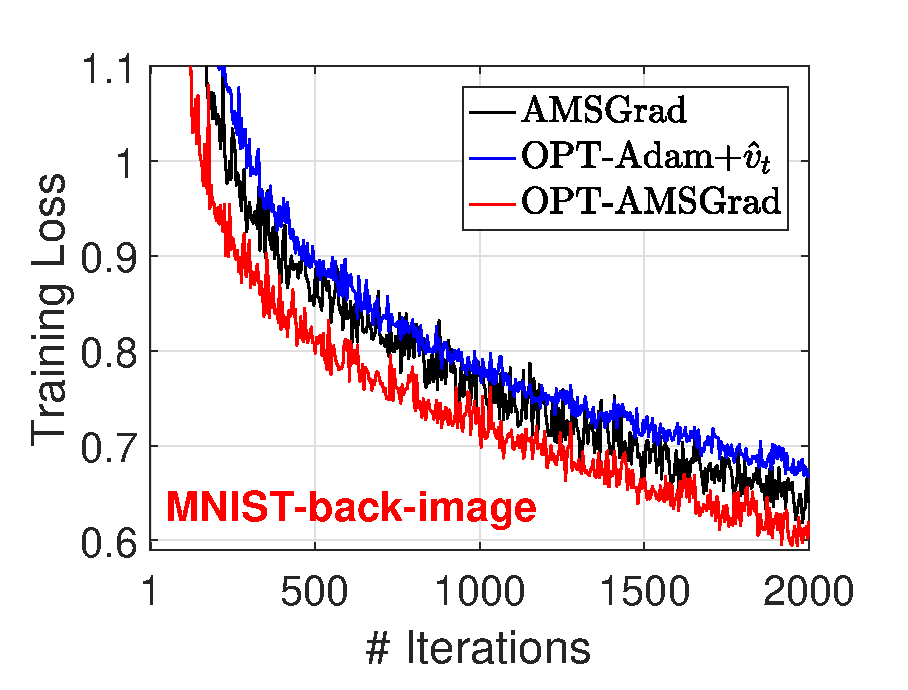
\includegraphics[width=0.94in]{simulation/fig2/M_image_train_loss_no1.eps}\hspace{-0.15in}
}
\subfigure{
\includegraphics[width=0.94in]{simulation/fig2/cifar_cnn_train_loss_no1.eps}\hspace{-0.15in}
}
\subfigure{
\includegraphics[width=0.94in]{simulation/fig2/imdb_lstm_train_loss_no1.eps}\hspace{-0.15in}
}
\subfigure{
\includegraphics[width=0.94in]{simulation/fig2/cifar10_resnet_train_loss.eps}\hspace{-0.15in}
}
\subfigure{
\includegraphics[width=0.94in]{simulation/fig2/cifar100_resnet_train_loss.eps}\hspace{-0.15in}
}
}
\caption{Training loss vs. Number of iterations. The first row are results with fully-connected NN.}
\label{fig:train_loss}
\end{figure}

\textbf{Datasets.}\hspace{0.1in}Following \cite{RKK18} and \cite{KB15}, we compare different algorithms on \textit{MNIST}, \textit{CIFAR10},
\textit{CIFAR100}, and \textit{IMDB} datasets. 
For \textit{MNIST}, we use two noisy variants named as 1.65\textit{MNIST-back-rand} and 1.65\textit{MNIST-back-image} from \cite{MNIST07}. They both have 12000 training samples and 50000 test samples, where random background is inserted to the original \textit{MNIST} hand written 
digit images. For \textit{MNIST-back-rand}, each image is inserted with a random background, whose pixel values generated uniformly from 0 to 255, while \textit{MNIST-back-image} takes random patches from a black and white as noisy background.
The input dimension is 784 ($28\times 28$) and the number of classes is $10$. \textit{CIFAR10} and \textit{CIFAR100} are popular computer-vision datasets consisting of 50000 training images and 10000 test images, of size $32\times 32$. The number of classes are 10 and 100, respectively. The \textit{IMDB} movie review dataset is a binary classification dataset with 25000 training and testing samples respectively. It is a popular datasets for text classification.

\textbf{Network architecture.}\hspace{0.1in}We adopt a multi-layer fully-connected neural network with input layer followed by a hidden layer with $200$ nodes, which is connected to another layer with $100$ nodes before the output layer. The activation function is ReLU for hidden layers, and softmax for the output layer. This network is tested on \textit{MNIST} variants. Since convolutional networks are popular for image classification tasks, we consider an ALL-CNN architecture proposed by \cite{CNN15}, which is constructed with several convolutional blocks and dropout layers. In addition, we also apply residual networks, Resnet-18 and Resnet-50~\cite{Rnet16}, which have achieved many state-of-the-art results. For the texture \textit{IMDB} dataset, we consider training a Long-Short Term Memory (LSTM) network. The network includes a word embedding layer with 5000 input entries representing most frequent words in the dataset, and each word is embedded into a 32 dimensional space. The output of the embedding layer is passed to 100 LSTM units, which is then connected to 100 fully connected ReLu's before the output layer. For all the models, we use cross-entropy loss. A mini-batch size of $128$ is used to compute the stochastic gradients.

\textbf{Results.}\hspace{0.1in}Firstly, to illustrate the acceleration effect of \textsc{OPTIMISTIC-AMSGrad} at early stage, we provide the training loss against number of iterations in Figure~\ref{fig:train_loss}. We clearly observe that on all datasets, the proposed \textsc{Optimistic-AMSGrad} converges faster than the other competing methods, right after the training begins. In other words, we need fewer iterations (samples) to achieve the same training loss. This validates one of the main advantages of \textsc{Optimistic-AMSGrad}, which is a higher sample efficiency.
We are also curious about the long-term performance and generalization of the proposed method in test phase. In Figure~\ref{fig:testandtrain}, we plot the corresponding results when the model is trained to the state with stable test accuracy. We observe: 1) In the long term, \textsc{OPTIMISTIC-AMSGrad} algorithm may converge to a better point with smaller objective function value, and 2) In this three applications, the proposed \textsc{OPTIMISTIC-AMSGrad} also outperforms the competing methods in terms of test accuracy. These are also important benefits of \textsc{OPTIMISTIC-AMSGrad}.


\begin{figure}[t]
\mbox{
\subfigure{
\includegraphics[width=0.94in]{new_figure/new_mnist_img_figure/mnist_img_train_loss_disz_2.eps}\hspace{-0.15in}
}
\subfigure{
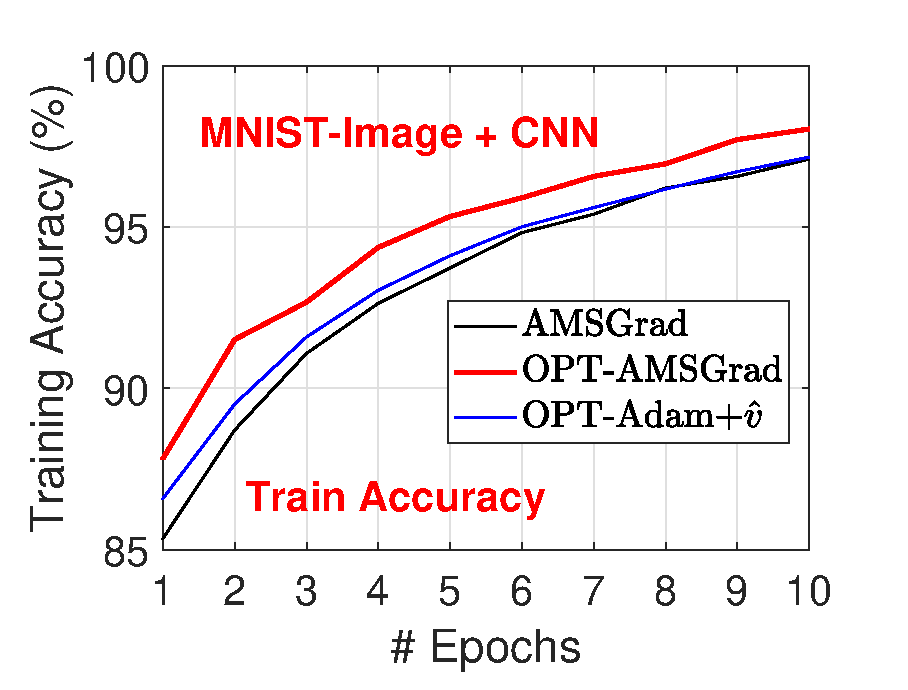
\includegraphics[width=0.94in]{new_figure/new_mnist_img_figure/mnist_img_train_acc_disz_2.eps}\hspace{-0.15in}
}
\subfigure{
\includegraphics[width=0.94in]{new_figure/mnist_img_test_loss_disz.eps}\hspace{-0.15in}
}
\subfigure{
\includegraphics[width=0.94in]{new_figure/mnist_img_test_acc_disz.eps}\hspace{-0.15in}
}
\subfigure{
\includegraphics[width=0.94in]{new_figure/cifar10_train_loss_disz.eps}\hspace{-0.15in}
}
\subfigure{
\includegraphics[width=0.94in]{new_figure/cifar10_train_acc_disz.eps}\hspace{-0.15in}
}
}
\mbox{
\subfigure{
\includegraphics[width=0.94in]{new_figure/cifar10_test_loss_disz.eps}\hspace{-0.15in}
}
\subfigure{
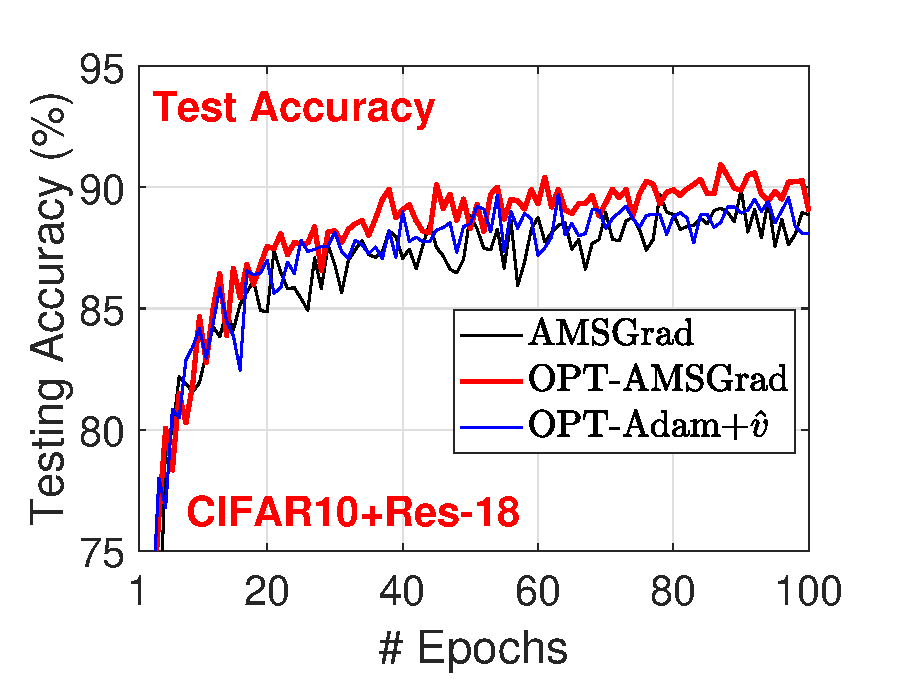
\includegraphics[width=0.94in]{new_figure/cifar10_test_acc_disz.eps}\hspace{-0.15in}
}
\subfigure{
\includegraphics[width=0.94in]{new_figure/cifar100_train_loss_disz.eps}\hspace{-0.15in}
}
\subfigure{
\includegraphics[width=0.94in]{new_figure/cifar100_train_acc_disz.eps}\hspace{-0.15in}
}
\subfigure{
\includegraphics[width=0.94in]{new_figure/cifar100_train_acc_disz.eps}\hspace{-0.15in}
}
\subfigure{
\includegraphics[width=0.94in]{new_figure/cifar100_test_acc_disz.eps}
}
}
\caption{\textit{MNIST-back-image} + CNN, \textit{CIFAR10} + Res-18 and \textit{CIFAR100} + Res-50 . We compare three methods in terms of training (cross-entropy) loss and accuracy, testing loss and accuracy.} \label{fig:testandtrain}
\end{figure}

\subsection{Choice of parameter $r$}
\begin{wrapfigure}[14]{r}{1.5in}\vspace{-0.3in}
\begin{center}
\mbox{
\includegraphics[width=1.35in]{new_figure/new_mnist_img_figure/mnist_img_train_loss_r3510_2.eps}\hspace{-0.1in}
}
\mbox{
\includegraphics[width=1.35in]{new_figure/cifar10_train_loss_r3510.eps}
}
\end{center}
\label{fig:compare}
\end{wrapfigure}
\vspace{-0.1in}
Recall that our proposed algorithm has the parameter $r$ that governs the use of past information.
Figure~\ref{fig:compare-r} compares the performance under different values of $r=3,5,10$ on two datasets. From the result we see that the choice of $r$ does not have significant impact on learning performance. Taking into consideration both quality of gradient prediction and computational cost, it appears that $r=5$ is a good choice. We remark that empirically, the performance comparison among $r=3,5,10$ is not absolutely consistent (i.e. more means better) in all cases. One possible reason is that for deep neural nets which have very complicated and highly non-convex landscape, using gradient information from too long ago may not be helpful in accurate gradient prediction. Nevertheless, $r=5$ seems to be good for most applications.

\subsection{Some Remarks on the Experiments}
\textbf{Discussion on the iteration cost:}
We observe that the iteration cost (i.e., actual running time per iteration) of our implementation of \textsc{Optimistic-AMSGrad} with $r=5$ is roughly two times larger than the standard \textsc{AMSGrad}. When $r=3$, the cost is roughly 0.7 times longer. Nevertheless, \textsc{OPTIMISTIC-AMSGrad} may still be beneficial in terms of training efficiency, since fewer iterations are typically needed. For example, in Figure \ref{figs:CIFAR10_new3} and \ref{figs:CIFAR100_new3}, to reach the training loss of \textsc{AMSGrad} at 100 epochs, the proposed method only needs roughly 20 and 40 epochs, respectively. That said, \textsc{OPTIMISTIC-AMSGrad} needs 40\% and 80\% time to achieve same training loss as \textsf{AMSGrad}, in this two problems.

The computational overhead mostly comes from the gradient extrapolation step. More specifically, recall that the extrapolation step consists of:
(a) The step of constructing the linear system $(U^\top U)$.
The cost of this step can be optimized and reduced to $\mathcal O(d)$, since the matrix $U$ only changes one column at a time.
(b) The step of solving the linear system.
The cost of this step is $O(r^3)$, which is negligible as the linear system is very small ($5$-by-$5$ if $r=5$).
(c) The step that outputs an estimated gradient as a weighted average of previous gradients.
The cost of this step is $\mathcal O(r \times d)$. Thus, the computational overhead is $\mathcal O\left((r+1)d+r^3\right)$.
Yet, we notice that step (a) and (c) is parallelizable, so they can be accelerated in practice.

\noindent \textbf{Memory usage:} Our algorithm needs a storage of past $r$ gradients for each coordinate, in addition to the estimated second moments and the moving average. Though it seems demanding compared to the standard AMSGrad, it is relatively cheap compared to Natural gradient method (e.g.,~\cite{MG15}), as Natural gradient method needs to store some matrix inverse.



\section{Conclusion}
In this paper, we propose \textsc{Optimistic-AMSGrad}, which combines optimistic learning and \textsc{AMSGrad} to improve sampling efficiency and
accelerate the process of training, in particular for deep neural networks. With a good gradient prediction, the regret can be smaller than that of standard \textsc{AMSGrad}. Experiments on various deep learning problems demonstrate the effectiveness of the proposed method in improving the training efficiency. 



\clearpage

\bibliographystyle{abbrvnat}
\bibliography{reference}

\clearpage


\appendix

\section{Proofs of Auxiliary Lemmas}
\subsection{Proof of Lemma~\ref{lem:bound}}\label{app:lembound}
\begin{Lemma*}
Assume assumption H~\ref{ass:bounded}, then the quantities defined in Algorithm~\ref{alg:optamsgrad} satisfy for any $w \in \Theta$ and $t>0$:
$$ \|\nabla f(w_t)\| < \major ,~~~\|\theta_t \| < \major ,~~~\|\hat{v}_t\| < \major^2 \eqsp.$$
\end{Lemma*}
\begin{proof}
Assume assumption H~\ref{ass:bounded} we have:
$$
\norm{\nabla f(w)} = \norm{\EE[\nabla f(w, \xi)]} \leq \EE[\norm{\nabla f(w, \xi)}] \leq \major
$$
By induction reasoning, since $\norm{\theta_0} = 0 \leq \major$ and suppose that for $\norm{\theta_t}\leq \major$ then we have 
\beq
\begin{split}
\norm{\theta_{t+1}}  =\norm{\beta_{1} \theta_{t}+\left(1-\beta_{1}\right) g_{t+1}} \leq \beta_1 \norm{\theta_{t}} + (1 - \beta_1) \norm{g_{t+1}} \leq \major
\end{split}
\eeq
Using the same induction reasoning we prove that
\beq
\begin{split}
\norm{\hat{v}_{t+1}}  =\norm{\beta_{2} \hat{v}_{t}+\left(1-\beta_{2}\right) g_{t+1}^2} \leq \beta_2 \norm{\hat{v}_{t}} + (1 - \beta_1) \norm{g^2_{t+1}} \leq \major^2
\end{split}
\eeq
\end{proof}

\subsection{Proof of Lemma~\ref{lem:momentum} }\label{app:lemmomentum}
\begin{Lemma*}
Assume a strictly positive and non increasing sequence of stepsizes $\{\eta_t \}_{t>0}$, $\beta_ \in [0,1]$, then the following holds:
\beq
\overline{w}_{t+1} - \overline{w}_t \leq \frac{\beta_1}{1 - \beta_1} \tilde{\theta}_{t-1} \left[ \eta_{t-1} \hat{v}_{t-1}^{-1/2} - \eta_{t} \hat{v}_{t}^{-1/2}\right] - \eta_{t} \hat{v}_{t}^{-1/2} \tilde{g}_t \eqsp,
\eeq
where $\tilde{\theta}_t = \theta_t + \beta_1 \theta_{t-1}$ and $\tilde{g}_t = g_t - \beta_1 m_t + \beta_1 g_{t-1} + m_{t+1} $.
\end{Lemma*}
\begin{proof}
By definition \eqref{eq:deftilde} and using the Algorithm updates, we have:
\beq
\begin{split}
\overline{w}_{t+1} - \overline{w}_t  &= \frac{1}{1 - \beta_1} ( w_{t+1} - w_t)  -  \frac{\beta_1}{1 - \beta_1}( w_{t} - w_{t-1})\\
& = - \frac{1}{1 - \beta_1} \eta_{t} \hat{v}_{t}^{-1/2} (\theta_t + h_{t+1})  +  \frac{\beta_1}{1 - \beta_1}\eta_{t-1} \hat{v}_{t-1}^{-1/2} (\theta_{t-1} + h_{t})\\
& = - \frac{1}{1 - \beta_1}  \eta_{t} \hat{v}_{t}^{-1/2} (\theta_t + \beta_1 \theta_{t-1}) -\frac{1}{1 - \beta_1}  \eta_{t} \hat{v}_{t}^{-1/2} (1- \beta_1) m_{t+1}\\
& + \frac{\beta_1}{1 - \beta_1} \eta_{t-1} \hat{v}_{t-1}^{-1/2} (\theta_{t-1} + \beta_1 \theta_{t-2}) + \frac{\beta_1}{1 - \beta_1}  \eta_{t-1} \hat{v}_{t-1}^{-1/2} (1- \beta_1) m_{t}
\end{split}
\eeq
Denote $\tilde{\theta}_t = \theta_t + \beta_1 \theta_{t-1}$ and $\tilde{g}_t = g_t - \beta_1 m_t + \beta_1 g_{t-1} + m_{t+1} $.
Notice that $\tilde{\theta}_t = \beta_1 \tilde{\theta}_{t-1} + (1 - \beta_1) (g_t + \beta_1 g_{t-1})$.
\beq
\begin{split}
\overline{w}_{t+1} - \overline{w}_t \leq \frac{\beta_1}{1- \beta_1} \tilde{\theta}_{t-1} \left[ \eta_{t-1} \hat{v}_{t-1}^{-1/2} - \eta_{t} \hat{v}_{t}^{-1/2} \right] - \eta_t \hat{v}_t^{-1/2} \tilde{g}_t
\end{split}
\eeq
\end{proof}

\subsection{Proof of Lemma~\ref{lem:squarev} }\label{app:lemsquarev}
\begin{Lemma*}
Assume H~\ref{ass:bounded}, a strictly positive and a sequence of constant stepsizes $\{\eta_t \}_{t>0}$, $\beta_ \in [0,1]$, then the following holds:
\beq
\sum_{t=1}^{T_{\sf max}} \eta_{t}^{2} \EE \left[\left\|\hat{v}_{t}^{-1/2} \theta_{t}\right\|_{2}^{2}\right] \leq  \frac{\eta^{2} d T_{\sf max} (1- \beta_1)}{(1 - \beta_2)(1-\gamma)} 
\eeq
\end{Lemma*}
\begin{proof}
We denote by index $p \in [1,d]$ the dimension of each component of vectors of interest. 
Noting that for any $t >0$ and dimension $p$ we have $\hat{v}_{t,p} \geq v_{t,p}$, then:
\beq
\begin{split}
\eta_{t}^{2} \EE \left[\left\|\hat{v}_{t}^{-1/2} \theta_{t}\right\|_{2}^{2}\right] &=\eta_{t}^{2} \mathbb{E}\left[\sum_{p=1}^{d} \frac{\theta_{t, p}^{2}}{\hat{v}_{t, p}}\right]  \\
& \leq \eta_{t}^{2} \mathbb{E}\left[\sum_{i=1}^{d} \frac{\theta_{t, p}^{2}}{v_{t, p}}\right] \\
& \leq \eta_{t}^{2} \mathbb{E}\left[\sum_{i=1}^{d} \frac{( \sum_{r=1}^t (1 - \beta_1) \beta_1^{t-r} g_{r,p})^{2}}{ \sum_{r=1}^t (1 - \beta_2) \beta_2^{t-r} g^2_{r,p}}\right] 
\end{split}
\eeq
where the last inequality is due to initializations.
Denote $\gamma = \frac{\beta_1}{\beta_2}$.
Then,
\beq
\begin{split}
\eta_{t}^{2} \EE \left[\left\|\hat{v}_{t}^{-1/2} \theta_{t}\right\|_{2}^{2}\right] &\leq \frac{\eta_{t}^{2} (1- \beta_1)^2}{1 - \beta_2}  \mathbb{E}\left[\sum_{i=1}^{d} \frac{( \sum_{r=1}^t \beta_1^{t-r} g_{r,p})^{2}}{ \sum_{r=1}^t \beta_2^{t-r} g^2_{r,p}}\right] \\
& \overset{(a)}{\leq}\frac{\eta_{t}^{2} (1- \beta_1)}{1 - \beta_2}  \mathbb{E}\left[\sum_{i=1}^{d} \frac{ \sum_{r=1}^t \beta_1^{t-r} g_{r,p}^{2}}{ \sum_{r=1}^t \beta_2^{t-r} g^2_{r,p}}\right]\\
& \leq \frac{\eta_{t}^{2} (1- \beta_1)}{1 - \beta_2}  \mathbb{E}\left[\sum_{i=1}^{d}\sum_{r=1}^t \gamma^{t-r}\right]  = \frac{\eta_{t}^{2} d (1- \beta_1)}{1 - \beta_2}  \mathbb{E}\left[\sum_{r=1}^t  \gamma^{t-r}\right] 
\end{split}
\eeq
where $(a)$ is due to $ \sum_{r=1}^t \beta_1^{t-r} \leq \frac{1}{1 - \beta_1}$.
Summing from  $t =1$ to $t = T_{\sf max}$ on both sides yields:
\beq
\begin{split}
\sum_{t=1}^{T_{\sf max}} \eta_{t}^{2} \EE \left[\left\|\hat{v}_{t}^{-1/2} \theta_{t}\right\|_{2}^{2}\right] &\leq   \frac{\eta_{t}^{2} d (1- \beta_1)}{1 - \beta_2}  \mathbb{E}\left[ \sum_{t=1}^{T_{\sf max}} \sum_{r=1}^t  \gamma^{t-r}\right]\\
& \leq  \frac{\eta^{2} d T (1- \beta_1)}{1 - \beta_2}  \mathbb{E}\left[ \sum_{t=t}^t   \gamma^{t-r}\right]\\
& \leq  \frac{\eta^{2} d T (1- \beta_1)}{(1 - \beta_2)(1-\gamma)} 
\end{split}
\eeq
where the last inequality is due to $\sum_{r=1}^t   \gamma^{t-r} \leq \frac{1}{1 - \gamma}$ by definition of $\gamma$.
\end{proof}



\section{Proofs of Theorem~\ref{thm:boundopt}}\label{app:thmboundopt}
\begin{Theorem*}
Assume H~\ref{ass:smooth}-H~\ref{ass:bounded}, $(\beta_1, \beta_2) \in [0,1]$ and a sequence of decreasing stepsizes $\{\eta_t\}_{t>0}$, then the following result holds:
\beq
\begin{split}
\EE\left[\|\nabla f(w_T)\|^2\right] \leq \tilde{C}_1 \sqrt{\frac{d}{T_{\sf max}}} + \tilde{C}_2 \frac{1}{T_{\sf max}}
\end{split}
\eeq
where $T$ is a random termination number distributed according \eqref{eq:random} and the constants are defined as follows:
\beq
\begin{split}
&\tilde{C}_1 = C_1 +  \frac{\major}{(1 - a\beta_1) + (\beta_1 + a)} \left[ \frac{a(1 - \beta_1)^2}{1-\beta_2} + 2L \frac{1}{1-\beta_2}  \right]\\
&C_1 = \frac{\major}{(1 - a\beta_1) + (\beta_1 + a)}  \Delta f + \frac{ 4L \left(\frac{\beta_1}{1 - \beta_1}\right)^2 \major}{(1 - a\beta_1) + (\beta_1 + a)} \frac{(1 + \beta_1^2) (1- \beta_1)}{(1 - \beta_2)(1-\gamma)}\\
&\tilde{C}_2 = \frac{\major}{(1 - \beta_1) \left((1 - a\beta_1) + (\beta_1 + a)\right)} \tilde{\major}^2   \EE\left[ \norm{\hat{v}_{0}^{-1/2}}    \right]
\end{split}
\eeq
\end{Theorem*}

\begin{proof}
Using H~\ref{ass:smooth} and the iterate $\overline{w}_t$ we have:
\beq\label{eq:smoothness}
\begin{split}
f(\overline{w}_{t+1}) & \leq  f(\overline{w}_t) + \nabla f(\overline{w}_t)^\top (\overline{w}_{t+1} - \overline{w}_t) + \frac{L}{2} \norm{\overline{w}_{t+1} - \overline{w}_t}^2\\
& \leq f(\overline{w}_t) + \underbrace{ \nabla f(w_t)^\top (\overline{w}_{t+1} - \overline{w}_t)}_{A} + \underbrace{  \left( \nabla f(\overline{w}_t) -  \nabla f(w_t)\right)^\top (\overline{w}_{t+1} - \overline{w}_t)}_{B} + \frac{L}{2} \norm{\overline{w}_{t+1} - \overline{w}_t}
\end{split}
\eeq

\textbf{Term A}.
Using Lemma~\ref{lem:momentum}, we have that:
\beq
\begin{split}
\nabla f(w_t)^\top (\overline{w}_{t+1} - \overline{w}_t) & \leq \nabla f(w_t)^\top \left[\frac{\beta_1}{1 - \beta_1} \tilde{\theta}_{t-1} \left[ \eta_{t-1} \hat{v}_{t-1}^{-1/2} - \eta_{t} \hat{v}_{t}^{-1/2}\right] - \eta_{t} \hat{v}_{t}^{-1/2} \tilde{g}_t \right]\\
& \leq  \frac{\beta_1}{1 - \beta_1}  \norm{ \nabla f(w_t)} \norm{\eta_{t-1} \hat{v}_{t-1}^{-1/2} - \eta_{t} \hat{v}_{t}^{-1/2} } \norm{\tilde{\theta}_{t-1}} - \nabla f(w_t)^\top\eta_{t} \hat{v}_{t}^{-1/2} \tilde{g}_t 
\end{split}
\eeq
where the inequality is due to trivial inequality for positive diagonal matrix.
Using Lemma~\ref{lem:bound} and assumption H\ref{ass:guessbound} we obtain:
\beq\label{eq:termA1}
\begin{split}
\nabla f(w_t)^\top (\overline{w}_{t+1} - \overline{w}_t)  \leq  \frac{\beta_1 (1+\beta_1)}{1 - \beta_1} \major^2 \left[ \norm{\eta_{t-1} \hat{v}_{t-1}^{-1/2}} - \norm{\eta_{t} \hat{v}_{t}^{-1/2} }\right] - \nabla f(w_t)^\top\eta_{t} \hat{v}_{t}^{-1/2} \tilde{g}_t 
\end{split}
\eeq
where we have used the fact that $\eta_{t} \hat{v}_{t}^{-1/2} $ is a diagonal matrix such that $\eta_{t-1} \hat{v}_{t-1}^{-1/2} \succcurlyeq \eta_{t} \hat{v}_{t}^{-1/2}\succcurlyeq 0$ (decreasing stepsize and $\max$ operator).
Also note that:
\beq\label{eq:termA2}
\begin{split}
 - \nabla f(w_t)^\top\eta_{t} \hat{v}_{t}^{-1/2} \tilde{g}_t  &=  - \nabla f(w_t)^\top\eta_{t-1} \hat{v}_{t-1}^{-1/2} \bar{g}_t   -  \nabla f(w_t)^\top\left[ \eta_{t} \hat{v}_{t}^{-1/2} -\eta_{t} \hat{v}_{t}^{-1/2} \right] \bar{g}_t  \\ 
&   - \nabla f(w_t)^\top\eta_{t-1} \hat{v}_{t-1}^{-1/2} (\beta_1 g_{t-1} + m_{t+1})\\
 & \leq  - \nabla f(w_t)^\top\eta_{t-1} \hat{v}_{t-1}^{-1/2} \bar{g}_t +(1-a\beta_1)\major^2    \left[ \norm{\eta_{t-1} \hat{v}_{t-1}^{-1/2}} - \norm{\eta_{t} \hat{v}_{t}^{-1/2} }\right] \\
 &  - \nabla f(w_t)^\top\eta_{t} \hat{v}_{t}^{-1/2} (\beta_1 g_{t-1} + m_{t+1})
\end{split}
\eeq
using Lemma~\ref{lem:bound} on $\norm{g_t}$ and where that $\tilde{g}_t = \bar{g}_t  + \beta_1 g_{t-1} + m_{t+1} = g_t - \beta_1 m_t + \beta_1 g_{t-1} + m_{t+1} $.
Plugging \eqref{eq:termA2} into \eqref{eq:termA1} yields:
\beq\label{eq:termA}
\begin{split}
&\nabla f(w_t)^\top (\overline{w}_{t+1} - \overline{w}_t)\\
&  \leq   - \nabla f(w_t)^\top\eta_{t-1} \hat{v}_{t-1}^{-1/2} \bar{g}_t + \frac{1}{1 - \beta_1} (a\beta_1^2 -2 a \beta_1 + \beta 1)\major^2 \left[ \norm{\eta_{t-1} \hat{v}_{t-1}^{-1/2}} - \norm{\eta_{t} \hat{v}_{t}^{-1/2} }\right] \\
&  - \nabla f(w_t)^\top\eta_{t} \hat{v}_{t}^{-1/2} (\beta_1 g_{t-1} + m_{t+1})
\end{split}
\eeq

\textbf{Term B}.
By Cauchy-Schwarz (CS) inequality we have:
\beq\label{eq:termB1}
 \left( \nabla f(\overline{w}_t) -  \nabla f(w_t)\right)^\top (\overline{w}_{t+1} - \overline{w}_t) \leq  \norm{ \nabla f(\overline{w}_t) -  \nabla f(w_t)}  \norm{\overline{w}_{t+1} - \overline{w}_t}
 \eeq
 Using smoothness assumption H~\ref{ass:smooth}:
\beq\label{eq:termB2}
 \begin{split}
  \norm{ \nabla f(\overline{w}_t) -  \nabla f(w_t)} & \leq L \norm{ \overline{w}_t - w_t}\\
  & \leq L \frac{\beta_1}{1 - \beta_1} \norm{w_t - w_{t-1}}
 \end{split}
 \eeq
By Lemma~\ref{lem:momentum} we also have:
 \beq
 \begin{split}
\overline{w}_{t+1} - \overline{w}_t & = \frac{\beta_1}{1 - \beta_1} \tilde{\theta}_{t-1} \left[ \eta_{t-1} \hat{v}_{t-1}^{-1/2} - \eta_{t} \hat{v}_{t}^{-1/2}\right] - \eta_{t} \hat{v}_{t}^{-1/2} \tilde{g}_t \\
& = \frac{\beta_1}{1 - \beta_1} \tilde{\theta}_{t-1}\eta_{t-1} \hat{v}_{t-1}^{-1/2} \left[ I - (\eta_{t} \hat{v}_{t}^{-1/2}) (\eta_{t-1} \hat{v}_{t-1}^{-1/2})^{-1} \right] - \eta_{t} \hat{v}_{t}^{-1/2} \tilde{g}_t \\
& = \frac{\beta_1}{1 - \beta_1} \left[ I - (\eta_{t} \hat{v}_{t}^{-1/2}) (\eta_{t-1} \hat{v}_{t-1}^{-1/2})^{-1} \right] (w_{t-1} - w_t) - \eta_{t} \hat{v}_{t}^{-1/2} \tilde{g}_t
 \end{split}
 \eeq
 where the last equality is due to $ \tilde{\theta}_{t-1}\eta_{t-1} \hat{v}_{t-1}^{-1/2} = w_{t-1} - w_t$ by construction of $\tilde{\theta}_t$.
 Taking the norms on both sides, observing $\norm{ I - (\eta_{t} \hat{v}_{t}^{-1/2}) (\eta_{t-1} \hat{v}_{t-1}^{-1/2})^{-1}} \leq 1$ due to the decreasing stepsize and the construction of $\hat{v}_t$ and using CS inequality yield:
\beq\label{eq:termB3}
 \begin{split}
\norm{\overline{w}_{t+1} - \overline{w}_t} & \leq \frac{\beta_1}{1 - \beta_1} \norm{w_{t-1} - w_t} + \norm{\eta_{t} \hat{v}_{t}^{-1/2} \tilde{g}_t}
 \end{split}
 \eeq 
 We recall Young's inequality with a constant $\delta \in (0,1)$ as follows:
$$
\pscal{X}{Y} \leq \frac{1}{\delta} \norm{X}^2 + \delta \norm{Y}^2
$$

 Plugging \eqref{eq:termB2} and \eqref{eq:termB3} into \eqref{eq:termB1} returns:
 \beq
 \begin{split}
 \left( \nabla f(\overline{w}_t) -  \nabla f(w_t)\right)^\top (\overline{w}_{t+1} - \overline{w}_t) \leq & L \frac{\beta_1}{1 - \beta_1} \norm{\eta_{t} \hat{v}_{t}^{-1/2} \tilde{g}_t}  \norm{w_t - w_{t-1}}\\
 & +  L\left(\frac{\beta_1}{1 - \beta_1} \right)^2 \norm{w_{t-1} - w_t}^2
  \end{split}
 \eeq
 
Applying Young's inequality with $\delta \to \frac{\beta_1}{1 - \beta_1}$ on the product $ \norm{\eta_{t} \hat{v}_{t}^{-1/2} \tilde{g}_t}  \norm{w_t - w_{t-1}}$ yields:
 \beq\label{eq:termB}
 \left( \nabla f(\overline{w}_t) -  \nabla f(w_t)\right)^\top (\overline{w}_{t+1} - \overline{w}_t) \leq  L \norm{\eta_{t} \hat{v}_{t}^{-1/2} \tilde{g}_t}^2 +  2L\left(\frac{\beta_1}{1 - \beta_1} \right)^2 \norm{w_{t-1} - w_t}^2
 \eeq
 
 The last term $ \frac{L}{2} \norm{\overline{w}_{t+1} - \overline{w}_t}$ can be upper bounded using \eqref{eq:termB3}:
\beq\label{eq:term3} 
\begin{split}
 \frac{L}{2} \norm{\overline{w}_{t+1} - \overline{w}_t}^2 & \leq  \frac{L}{2} \left[ \frac{\beta_1}{1 - \beta_1} \norm{w_{t-1} - w_t} + \norm{\eta_{t} \hat{v}_{t}^{-1/2} \tilde{g}_t}\right]\\
 &  \leq L \norm{\eta_{t} \hat{v}_{t}^{-1/2} \tilde{g}_t}^2 + 2L  \left(\frac{\beta_1}{1 - \beta_1}\right)^2 \norm{w_{t-1} - w_t}^2 
\end{split}
\eeq


Plugging \eqref{eq:termA}, \eqref{eq:termB} and \eqref{eq:term3} into \eqref{eq:smoothness} and taking the expectations on both sides give:
\beq
\begin{split}
& \EE\left[f(\overline{w}_{t+1})  +   \frac{1}{1 - \beta_1}\tilde{\major}^2  \norm{\eta_{t} \hat{v}_{t}^{-1/2} }  - \left( f(\overline{w}_{t}) + \frac{1}{1 - \beta_1}\tilde{\major}^2 \norm{\eta_{t-1} \hat{v}_{t-1}^{-1/2}} \right)        \right] \\
& \leq \EE \left[ - \nabla f(w_t)^\top\eta_{t-1} \hat{v}_{t-1}^{-1/2} \bar{g}_t  - \nabla f(w_t)^\top\eta_{t} \hat{v}_{t}^{-1/2} ( \beta_1 g_{t-1} +m_{t+1})   \right]\\
& + \EE \left[ 2L \norm{\eta_{t} \hat{v}_{t}^{-1/2} \tilde{g}_t}^2 + 4L  \left(\frac{\beta_1}{1 - \beta_1}\right)^2 \norm{w_{t-1} - w_t}^2  \right]
\end{split}
\eeq
where $ \tilde{\major}^2 = (a\beta_1^2 -2 a \beta_1 + \beta 1)\major^2$.
Note that the expectation of $ \tilde{g}_t $ conditioned on the filtration $\mathcal{F}_{t}$ reads as follows
\beq\label{eq:expectationtildegrad}
\begin{split}
\EE\left[    \nabla f(w_t)^\top \bar{g}_t  \right] & = \EE\left[  \nabla  f(w_t)^\top (g_t  - \beta_1 m_{t})  \right]\\
& = (1-a\beta_1) \| \nabla f(w_t) \|^2
\end{split}
\eeq
Summing from $t=1$ to $t=T$ leads to 
\beq\label{eq:bound1}
\begin{split}
& \frac{1}{\major} \sum_{t=1}^{T_{\sf max}} \left( (1 - a\beta_1)   \eta_{t-1} + (\beta_1 + a)   \eta_{t} \right) \norm{\nabla f(w_t)}^2 \leq\\
&  \EE\left[  f(\overline{w}_{1}) + \frac{1}{1 - \beta_1}\tilde{\major}^2 \norm{\eta_{0} \hat{v}_{0}^{-1/2}}    - \left(f(\overline{w}_{T_{\sf max}+1})  +   \frac{1}{1 - \beta_1}\tilde{\major}^2  \norm{\eta_{T_{\sf max}} \hat{v}_{T_{\sf max}}^{-1/2} } \right)      \right]\\
& +2L  \sum_{t=1}^{T_{\sf max}}  \EE \left[  \norm{\eta_{t} \hat{v}_{t}^{-1/2} \tilde{g}_t}^2 \right] + 4L \left(\frac{\beta_1}{1 - \beta_1}\right)^2 \sum_{t=1}^{T_{\sf max}}  \EE \left[  \norm{w_{t-1} - w_t}^2  \right]\\
& \leq  \EE\left[  \Delta f  + \frac{1}{1 - \beta_1}\tilde{\major}^2 \norm{\eta_{0} \hat{v}_{0}^{-1/2}}    \right] +2L  \sum_{t=1}^{T_{\sf max}}  \EE \left[  \norm{\eta_{t} \hat{v}_{t}^{-1/2} \tilde{g}_t}^2 \right] + 4L \left(\frac{\beta_1}{1 - \beta_1}\right)^2 \sum_{t=1}^{T_{\sf max}}  \EE \left[  \norm{w_{t-1} - w_t}^2  \right]\\
\end{split}
\eeq
where $ \Delta f = f(\overline{w}_{1}) - f(\overline{w}_{T_{\sf max}+1})$.
We note that by definition of $\hat{v}_t$, and a constant learning rate $\eta_t$, we have
\beq
\begin{split}
\norm{w_{t-1} - w_t}^2 & =\norm{\eta_{t-1} \hat{v}_{t-1}^{-1/2} (\theta_{t-1} + h_{t})}^2 \\
& =\norm{\eta_{t-1} \hat{v}_{t-1}^{-1/2} (\theta_{t-1} + \beta_{1} \theta_{t-2} + (1-\beta_{1}) m_{t})}^2\\
& \leq \norm{\eta_{t-1} \hat{v}_{t-1}^{-1/2}\theta_{t-1}}^2 + \norm{\eta_{t-2} \hat{v}_{t-2}^{-1/2} \beta_{1} \theta_{t-2}}^2 + (1-\beta_{1})^2 \norm{\eta_{t-1} \hat{v}_{t-1}^{-1/2}m_{t}}^2
\end{split}
\eeq
Using Lemma~\ref{lem:squarev} we have
\beq
\begin{split}
& \sum_{t=1}^{T_{\sf max}} \EE \left[  \norm{w_{t-1} - w_t}^2  \right]\\ 
& \leq (1 + \beta_1^2) \frac{\eta^{2} d T_{\sf max} (1- \beta_1)}{(1 - \beta_2)(1-\gamma)} + (1 - \beta_1)^2 \sum_{t=1}^{T_{\sf max}} \EE \left[ \norm{\eta_{t-1} \hat{v}_{t-1}^{-1/2}m_{t}}^2\right]
\end{split}
\eeq
And thus, setting the learning rate to a constant value $\eta$ and injecting in \eqref{eq:bound1} yields:
\beq
\begin{split}
&\EE\left[\|\nabla f(w_T)\|^2\right] = \frac{ 1 }{\sum_{j=1}^{T_{\sf max}} \eta_j}  \sum_{t=1}^{T_{\sf max}} \eta_{t} \norm{\nabla f(w_t)}^2 \\
& \leq \frac{\major}{(1 - a\beta_1) + (\beta_1 + a)}  \frac{ 1 }{\sum_{j=1}^{T_{\sf max}} \eta_j}   \EE\left[  \Delta f  + \frac{1}{1 - \beta_1}\tilde{\major}^2 \norm{\eta_{0} \hat{v}_{0}^{-1/2}}    \right]\\
& +  \frac{ 4L \left(\frac{\beta_1}{1 - \beta_1}\right)^2 \major}{(1 - a\beta_1) + (\beta_1 + a)}  \frac{ 1 }{\sum_{j=1}^{T_{\sf max}} \eta_j}  (1 + \beta_1^2) \frac{\eta^{2} d T_{\sf max} (1- \beta_1)}{(1 - \beta_2)(1-\gamma)}\\
& + \frac{\major}{(1 - a\beta_1) + (\beta_1 + a)}  \frac{ 1 }{\sum_{j=1}^{T_{\sf max}} \eta_j} (1 - \beta_1)^2 \sum_{t=1}^{T_{\sf max}} \EE \left[ \norm{\eta_{t-1} \hat{v}_{t-1}^{-1/2}m_{t}}^2\right]\\
& +  \frac{2L\major}{(1 - a\beta_1) + (\beta_1 + a)}  \frac{ 1 }{\sum_{j=1}^{T_{\sf max}} \eta_j}   \sum_{t=1}^{T_{\sf max}}  \EE \left[  \norm{\eta_{t} \hat{v}_{t}^{-1/2} \tilde{g}_t}^2 \right] 
\end{split}
\eeq
where $T$ is a random termination number distributed according \eqref{eq:random}.
Setting the stepsize to $\eta = \frac{1}{\sqrt{d T_{\sf max}}}$ yields :
\beq
\begin{split}
&\EE\left[\|\nabla f(w_T)\|^2\right]\\
& \leq C_1 \sqrt{\frac{d}{T_{\sf max}}} + C_2 \frac{1}{T_{\sf max}}\\
& + D_1 \frac{\eta}{T_{\sf max}} \sum_{t=1}^{T_{\sf max}} \EE \left[ \norm{ \hat{v}_{t-1}^{-1/2}m_{t}}^2\right] + D_2 \frac{\eta}{T_{\sf max}} \sum_{t=1}^{T_{\sf max}} \EE \left[ \norm{ \hat{v}_{t-1}^{-1/2} \tilde{g}_{t}}^2\right] 
\end{split}
\eeq
where
\beq
\begin{split}
&C_1 = \frac{\major}{(1 - a\beta_1) + (\beta_1 + a)}  \Delta f + \frac{ 4L \left(\frac{\beta_1}{1 - \beta_1}\right)^2 \major}{(1 - a\beta_1) + (\beta_1 + a)} \frac{(1 + \beta_1^2) (1- \beta_1)}{(1 - \beta_2)(1-\gamma)} \\
&C_2 =\frac{\major}{(1 - \beta_1) \left((1 - a\beta_1) + (\beta_1 + a)\right)} \tilde{\major}^2   \EE\left[ \norm{\hat{v}_{0}^{-1/2}}    \right]
\end{split}
\eeq

\textbf{Simple case as in \citep{zhou2018convergence}:} if $\beta_1 = 0$ then $ \tilde{g}_{t} = g_t + m_{t+1}$ and $g_t = \theta_t$. Also using Lemma~\ref{lem:squarev} we have that:
\beq
\sum_{t=1}^{T_{\sf max}} \eta_{t}^{2} \EE \left[\left\|\hat{v}_{t}^{-1/2} g_{t}\right\|_{2}^{2}\right] \leq  \frac{\eta^{2} d T_{\sf max}}{(1 - \beta_2)} 
\eeq
which leads to the final bound:
\beq
\begin{split}
&\EE\left[\|\nabla f(w_T)\|^2\right]\\
& \leq \tilde{C}_1 \sqrt{\frac{d}{T_{\sf max}}} + \tilde{C}_2 \frac{1}{T_{\sf max}}
\end{split}
\eeq
where
\beq
\begin{split}
&\tilde{C}_1 = C_1 +  \frac{\major}{(1 - a\beta_1) + (\beta_1 + a)} \left[ \frac{a(1 - \beta_1)^2}{1-\beta_2} + 2L \frac{1}{1-\beta_2}  \right]\\
&\tilde{C}_2 = C_2 =\frac{\major}{(1 - \beta_1) \left((1 - a\beta_1) + (\beta_1 + a)\right)} \tilde{\major}^2   \EE\left[ \norm{\hat{v}_{0}^{-1/2}}    \right]
\end{split}
\eeq
\end{proof}

\section{Proof of Lemma~\ref{lem:dnnh2} (Boundedness of the iterates)}\label{app:lemdnnh2}
\begin{Lemma*}
Given the multilayer model \eqref{eq:dnnmodel}, assume the boundedness of the input data and of the loss function, \ie for any $\xi \in \rset^l$ and $y \in \rset$ there is a constant $T >0$ such that:
\beq\label{eq:mildassumptions}
\norm{\xi} \leq 1 \quad \textrm{a.s.} \quad \textrm{and} |\mathcal{L}'(\cdot, y)| \leq T
\eeq
where $\mathcal{L}'(\cdot, y)$ denotes its derivative \wrt the parameter. Then for each layer $\ell \in [1,L]$, there exist a constant $A_{(\ell)}$ such that:
$$
\norm{w^{(\ell)}} \leq A_{(\ell)}
$$
\end{Lemma*}
\begin{proof}
Recall that for any layer index $\ell \in [1, L]$ we denote the output of layer $\ell$ by $h^{(\ell)}(w,\xi)$:
$$
h^{(\ell)}(w,\xi) = \sigma\left(w^{(\ell)} \sigma\left(w^{(\ell-1)} \ldots \sigma\left(w^{(1)} \xi \right)\right)\right)
$$
Given the sigmoid assumption we have $\norm{h^{(\ell)}(w,\xi)} \leq 1$ for any $\ell \in [1,L]$ and any $(w, \xi) \in \rset^d \times \rset^l$.
Observe that at the last layer $L$:
\beq\label{eq:boundderivativeloss}
\begin{split}
\norm{\nabla_{w^{(L)}}  \mathcal{L}(\textsf{MLN}( w, \xi), y)} & =  \norm{\mathcal{L}'(\textsf{MLN}( w, \xi), y)\nabla_{w^{(L)}}\textsf{MLN}( w, \xi)}\\
&  = \norm{\mathcal{L}'(\textsf{MLN}( w, \xi), y)\sigma'(w^{(L)} h^{(L-1)}(w,\xi))h^{(L-1)}(w,\xi)}\\
& \leq \frac{T}{4}
\end{split}
\eeq
where the last equality is due to mild assumptions \eqref{eq:mildassumptions} and to the fact that the norm of the derivative of the sigmoid function is upperbounded by $1/4$.

From Algorithm~\ref{alg:optamsgrad}, with $\beta_1 = 0$ we have for iteration index $t >0$:
\beq
\begin{split}
\norm{w_t - w_{t-1}} & = \norm{-\eta_t \hat{v}_t^{-1/2} (\theta_t + h_{t+1})}\\
&  = \norm{\eta_t \hat{v}_t^{-1/2} (g_t + m_{t+1})}\\
& \leq \hat{\eta} \norm{\hat{v}_t^{-1/2} g_t} + \hat{\eta} a \norm{\hat{v}_t^{-1/2} g_{t+1}}
\end{split}
\eeq
where $\hat{\eta} = \max \limits_{t >0} \eta_t$.
For any dimension $p \in [1,d]$, using assumption H~\ref{ass:guessbound}, we note that 
$$\sqrt{\hat{v}_{t,p}} \geq \sqrt{1-\beta_2} g_{t,p} \quad \textrm{and} \quad m_{t+1} \leq  a \norm{g_{t+1}}$$ .
Thus:
\beq
\begin{split}
\norm{w_t - w_{t-1}} & \leq \hat{\eta} \left( \norm{\hat{v}_t^{-1/2} g_t} +  a \norm{\hat{v}_t^{-1/2} g_{t+1}} \right) \\
& \leq \hat{\eta} \frac{a +1}{\sqrt{1 - \beta_2}} 
\end{split}
\eeq
In short there exist a constant $B$ such that $\norm{w_t - w_{t-1}} \leq B$.

\textbf{Proof by induction:} As in \citep{defossez2020convergence}, we will prove the containment of the weights by induction.
Suppose an iteration index $T$ and a coordinate $i$ of the last layer $L$ such that $w^{(L)}_{T, i} \geq \frac{T}{4\lambda} + B$.
Using \eqref{eq:boundderivativeloss}, we have
$$
\nabla_i f(w^{(L)}_t\geq - \frac{T}{4} + \lambda \frac{T}{\lambda4} \geq 0
$$
where $f(\cdot)$ is defined by \eqref{eq:lossmln} and is the loss of our MLN.
This last equation yields $\theta^{(L)}_{T,i} \geq 0$ (given the algorithm and $\beta_1 = 0$) and using the fact that $\norm{w_t - w_{t-1}} \leq B$ we have
\beq\label{eq:decrease}
0 \leq w^{(L)}_{T-1,i} - B \leq w^{(L)}_{T,i} \leq w^{(L)}_{T-1,i}
\eeq
which means that $| w^{(L)}_{T,i}| \leq w^{(L)}_{T-1,i}$.
So if the first assumption of that induction reasoning holds, \ie $w^{(L)}_{T-1, i} \geq \frac{T}{4\lambda} + B$, then the next iterates $w^{(L)}_{T, i}$ decreases, see \eqref{eq:decrease} and go below $\frac{T}{4\lambda} + B$. This yields that for any iteration index $t >0$ we have 
$$
w^{(L)}_{T, i} \leq \frac{T}{4\lambda} + 2B
$$
since $B$ is the biggest jump an iterate can do since $\norm{w_t - w_{t-1}} \leq B$.
Likewise we can end up showing that 
$$
|w^{(L)}_{T, i}| \leq \frac{T}{4\lambda} + 2B
$$
meaning that the weights of the last layer at any iteration is bounded in some matrix norm.

Now that we have shown this boundedness property for the last layer $L$, we will do the same for the previous layers and conclude the verification of assumption H~\ref{ass:boundedparam} by induction.

For any layer $\ell \in [1, L-1]$, we have:
\beq\label{eq:gradientatell}
\nabla_{w^{(\ell)}}  \mathcal{L}(\textsf{MLN}( w, \xi), y)  =  \mathcal{L}'(\textsf{MLN}( w, \xi), y) \left(\prod_{j=1}^{\ell+1} \sigma'\left(w^{(j)} h^{(j-1)}(w,\xi) \right) \right) h^{(\ell-1)}(w,\xi) 
\eeq
This last quantity is bounded as long as we can prove that for any layer $\ell$ the weights $w^{(\ell)}$ are bounded in some matrix norm as $\norm{w^{(\ell)}}_{F} \leq F_\ell$ with the Frobenius norm.
Suppose we have shown $\norm{w^{(r)}}_{F} \leq F_r$ for any layer $r > \ell$. 
Then having this gradient \eqref{eq:gradientatell} bounded we can use the same lines of proof for the last layer $L$ and show that the norm of the weights at the selected layer $\ell$ satisfy
$$
\norm{w^{(\ell)}} \leq \frac{T \prod_{t > \ell} F_t}{4^{L-\ell+1}} + 2B
$$
Showing that the weights of the previous layers $\ell \in [1, L-1]$ as well as for the last layer $L$ of our fully connected feed forward neural network are bounded at each iteration, leads by induction, to the boundedness (at each iteration) assumption we want to check.
\end{proof}

%-----------------------------------------------------------------------------
%\vspace{0.4cm}

\end{document} 
